\documentclass[%
%handout, % prints handouts (=no animations, for printed version)
%mathserif
%xcolor=pst,
14pt
%fleqn
]{beamer}

\usepackage{beamerthemedefault}

\useoutertheme[subsection=false]{smoothbars}
\useinnertheme[shadow=true]{rounded}

\setbeamercolor{block title}{fg=black,bg=gray}
\setbeamercolor{block title alerted}{use=alerted text,fg=black,bg=alerted text.fg!75!bg}
\setbeamercolor{block title example}{use=example text,fg=black,bg=example text.fg!75!bg}
\setbeamercolor{block body}{parent=normal text,use=block title,bg=block title.bg!25!bg}
\setbeamercolor{block body alerted}{parent=normal text,use=block title alerted,bg=block title alerted.bg!25!bg}
\setbeamercolor{block body example}{parent=normal text,use=block title example,bg=block title example.bg!25!bg}

%% for including video/audio
%\usepackage{multimedia} %needs hyperref-package
%\usepackage{movie15}

%\usepackage{xmpmulti}

%% aktive Referenzen
%\usepackage{hyperref}

%\usepackage{ngerman}			% language set to new-german
\usepackage[english]{babel}			% language set to new-german
\usepackage[utf8]{inputenc} 	% coding of german special characters
% \usepackage{ae,aecompl}
\usepackage{amsmath,amssymb,amstext} 	% support for mathematics

% \usepackage{listings}		% include programming code
%\usepackage{amsfonts}		% blackboard fonts: $\mathbb{N,Z,R,C,...}$
%\usepackage{latexsym}
%\usepackage{textcomp}
%\usepackage{mathptmx,courier}
			% \textdegree \textcelsius \textperthousand
			% \copyright \texttrademark \textregistered
			% \textmu (non-italic mu)
%\usepackage{geometry}	% change paper dimension an margins
%    \geometry{verbose,paperwidth=128mm,paperheight=90mm}
%    \geometry{tmargin=0mm,bmargin=0mm,lmargin=10mm,rmargin=10mm}
\usepackage[]{graphicx}  % \includegraphics[options]{file.eps}
\usepackage{subfigure}
			% options = scale, width, totalheight, height, depth,
			% angle = deg, origin = {l c r}{top, Baseline, bottom}
			% \scalebox{h-scale}[v-scale]{object}
			% \rotatebox[x=xdim,y=ydim]{angleCCW}[object}
%\usepackage{tabularx}	% \begin{tabular}{...X...} stretches column
%\usepackage{multirow}
%\usepackage{floatflt}
%\usepackage{hhline}
%\usepackage{colortbl}
\usepackage{array}
\usepackage{setspace}

\usepackage{tikz}
\usetikzlibrary{arrows,positioning}

%\usepackage[thinspace,thinqspace,squaren,textstyle]{SIunits}

\definecolor{tug}{rgb}{0.96862,0.14509,0.27450}

\setbeamertemplate{headline}[text line]{
	\begin{beamercolorbox}[wd=\paperwidth,ht=8ex,dp=4ex]{}
		\insertnavigation{0.85\paperwidth} 
		\raisebox{-10pt}{\includegraphics[width=15mm]{tuglogo}}\vskip2pt
		\hskip-1pt\rule{\paperwidth}{0.3pt}
	\end{beamercolorbox}
}

\setbeamertemplate{navigation symbols}{}

\definecolor{gray}{rgb}{0.8,0.8,0.8}
\setbeamercolor{footline}{fg=black,bg=gray}

% Fußzeile mit Autor, Titel und Foliennummer / Gesamtfolienzahl
\setbeamertemplate{footline}[text line]{
	\hskip-1pt
	\begin{beamercolorbox}[wd=\paperwidth]{footline}
			\rule{\paperwidth}{0.3pt}
			\colorbox{tug}{\rule{3pt}{0pt}\rule{0pt}{3pt}}
			\textbf{\rule{0pt}{5pt}\insertshortauthor\hfill\insertshortinstitute\hfill%
					\insertshorttitle\rule{1em}{0pt}}
			\rule{\paperwidth}{0.3pt}
	\end{beamercolorbox}
	\begin{beamercolorbox}[wd=\paperwidth,ht=2ex,dp=2ex]{white}
	\end{beamercolorbox}
}%
\usepackage{xspace}

%% Titelblatt-Einstellungen
%\institute[TU Graz]{Institute of Medical Engineering, TU Graz }
\title{EyeTracking with two cameras}
\subtitle{Image Processing and Pattern Recognition Project}
\author{Christoph Aigner, Stefan Kroboth}
\date{January 23, 2012}		% wenn ein anderes als das heutige Datum eingesetzt werden soll

% Subject und Keywords für PDF-Datei
\subject{EyeTracking with two cameras}
\keywords{EyeTracking, Eye, Pupil, Tracking}

\titlegraphic{\includegraphics[width=20mm]{tuglogo}}

%%%%%%%%%%%%%%%%%%%%%%%%%%%%%%%%%%%%%%%%%%%%%%%%%%%%%%%%%%%%%%%%%%%%%%%%%%%%
\begin{document}
%%%%%%%%%%%%%%%%%%%%%%%%%%%%%%%%%%%%%%%%%%%%%%%%%%%%%%%%%%%%%%%%%%%%%%%%%%%%

\begin{frame}[plain]
  \frametitle{}
  \titlepage % erzeugt Titelseite
\end{frame}



\begin{frame}
  \frametitle{Contents}
  \begin{spacing}{0.7}
        \tableofcontents[hideallsubsections %
                        % ,pausesections
                        ] % erzeugt Inhaltsverzeichnis
                      \end{spacing}
\end{frame}

%%%%%%%%%%%%%%%%%%%%%%%%%%%%%%%%%%%%%%%%%%%%%%%%%%%%%%%%%%%%%%%%%%%%%%%%%%%%
\section{Introduction}
%%%%%%%%%%%%%%%%%%%%%%%%%%%%%%%%%%%%%%%%%%%%%%%%%%%%%%%%%%%%%%%%%%%%%%%%%%%%
\subsection{Introduction}
\begin{frame}
	\frametitle{Introduction}
  \begin{itemize}
    \item Goal: Map eye movement onto screen independent of head position
    \item two cameras
      \begin{itemize}
        \item eye camera $\rightarrow$ track eye movement
        \item head camera $\rightarrow$ track head movement
      \end{itemize}
  \end{itemize}
\end{frame}

\section{Methods}
\subsection{Hardware}
\begin{frame}
	\frametitle{Hardware}
  %\framesubtitle{Reconstruction}
  \vspace*{-0.5cm}
  \begin{center}
    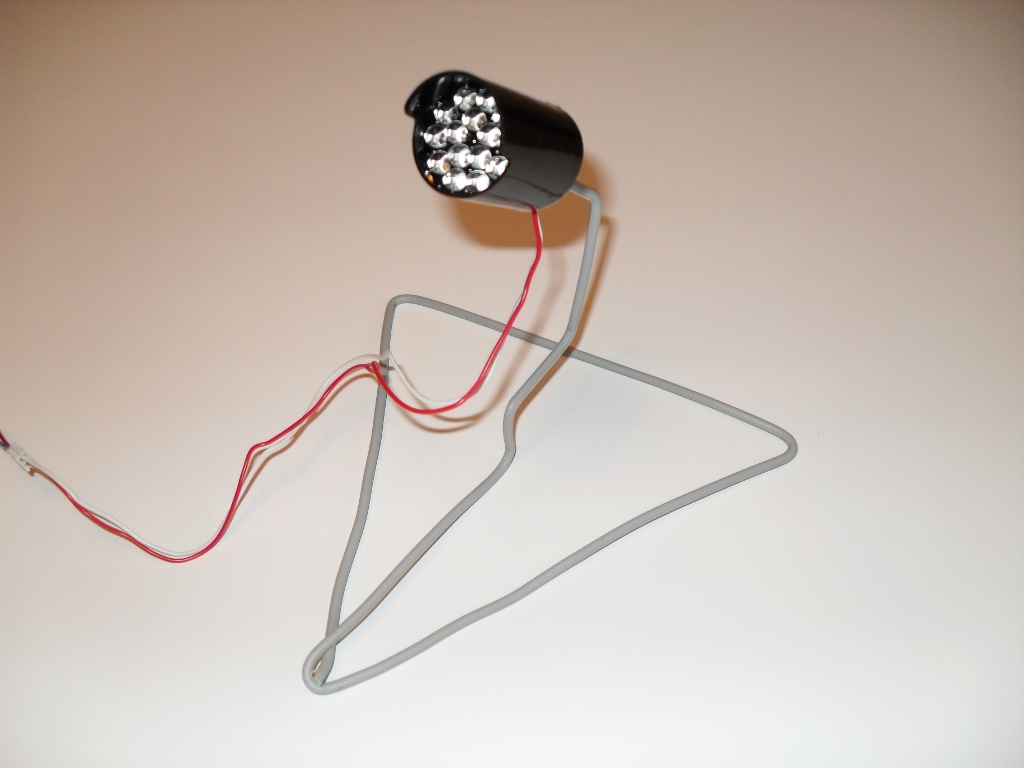
\includegraphics[width=0.4\textwidth]{SDC11117.JPG}
    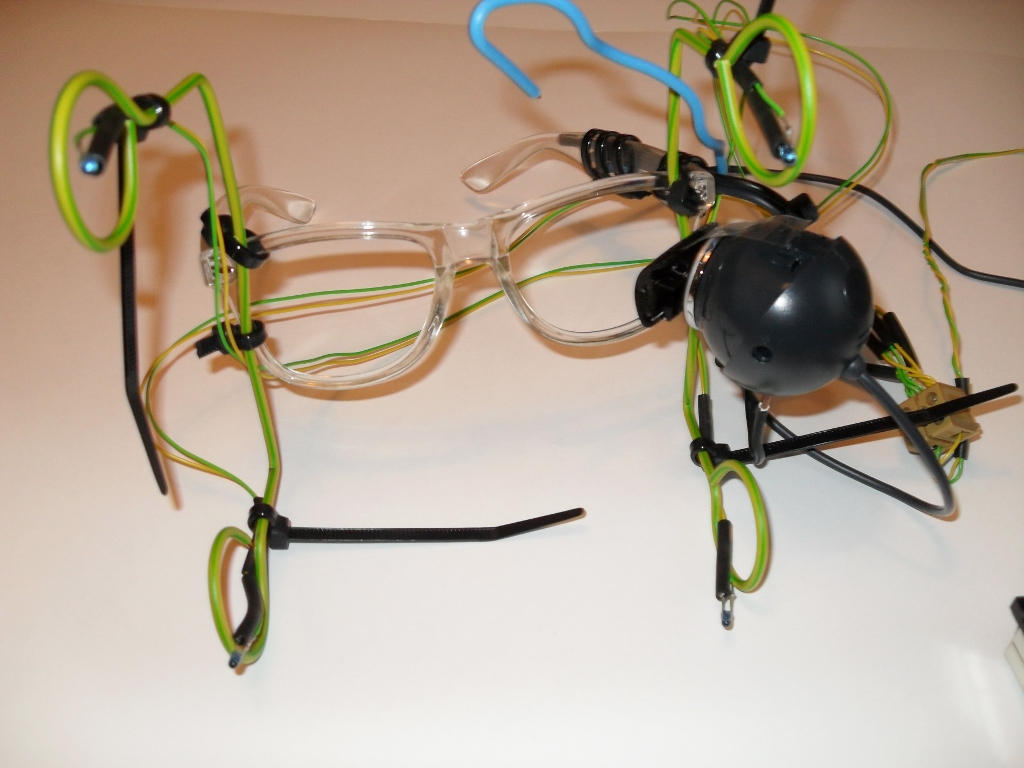
\includegraphics[width=0.4\textwidth]{SDC11119.JPG}\\
    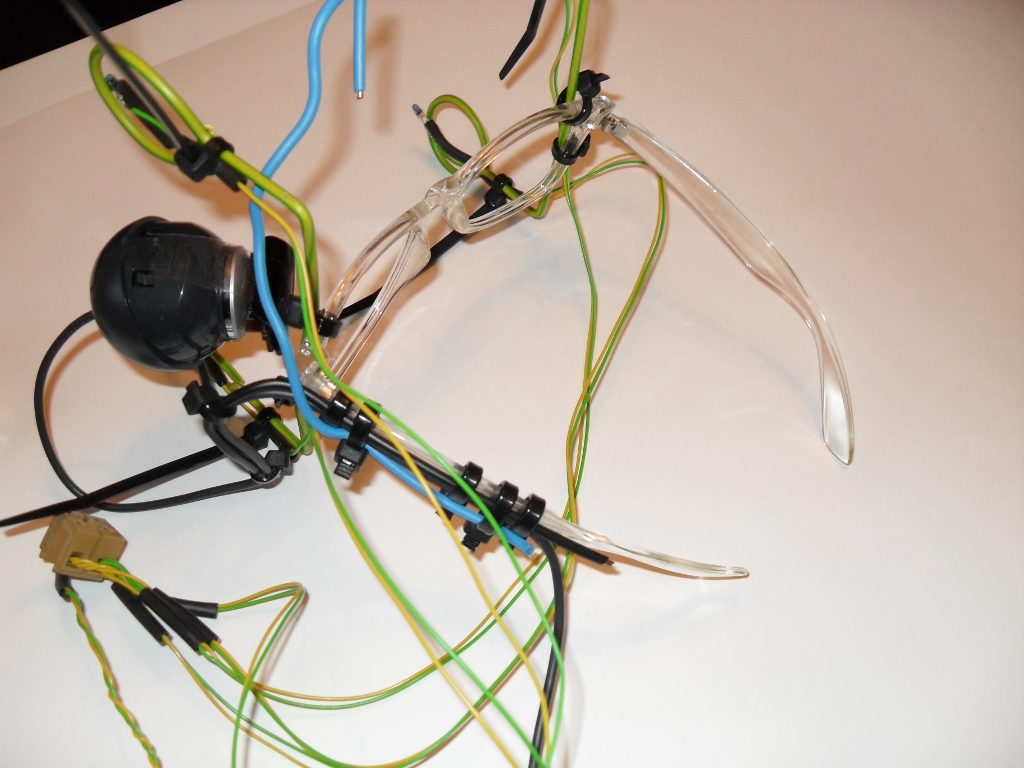
\includegraphics[width=0.4\textwidth]{SDC11121.JPG}
    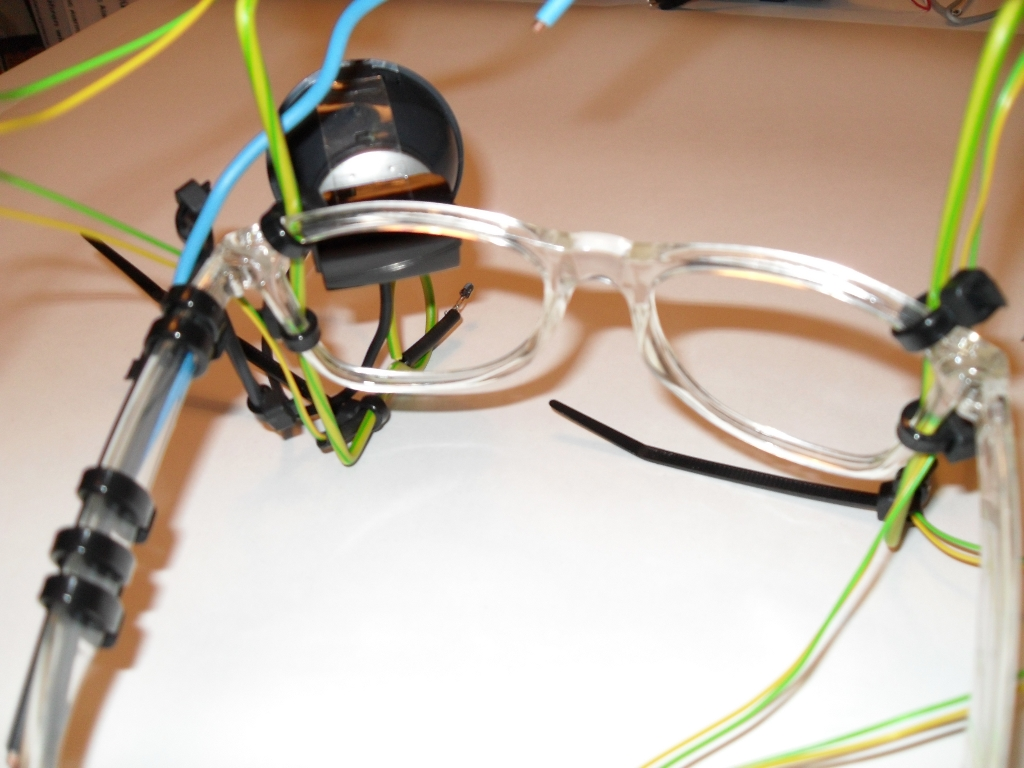
\includegraphics[width=0.4\textwidth]{SDC11122.JPG}
  \end{center}

\end{frame}

\subsection{Software}
\begin{frame}
	\frametitle{Software}
  \framesubtitle{Idea}
  \vspace*{-0.5cm}
  \begin{center}
    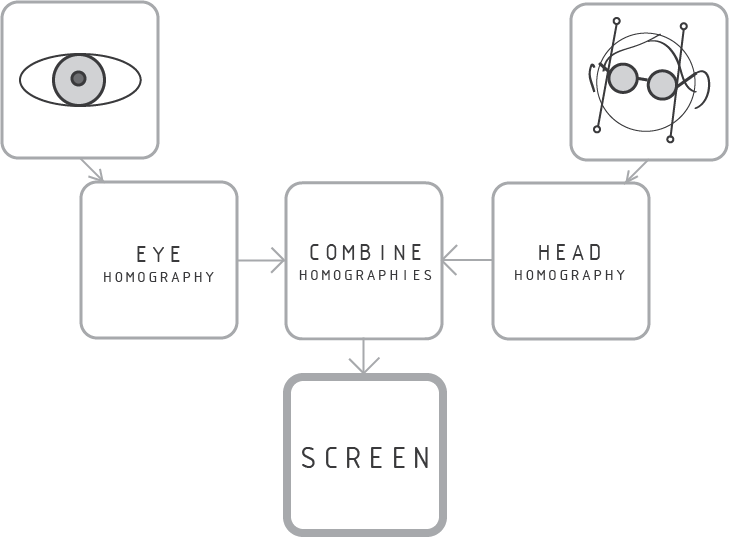
\includegraphics[width=0.8\textwidth]{01.png}
  \end{center}

\end{frame}
\subsubsection{Head Tracking}
\begin{frame}
	\frametitle{Software}
  \framesubtitle{Head Tracking}
  \vspace*{-0.5cm}
  \begin{center}
    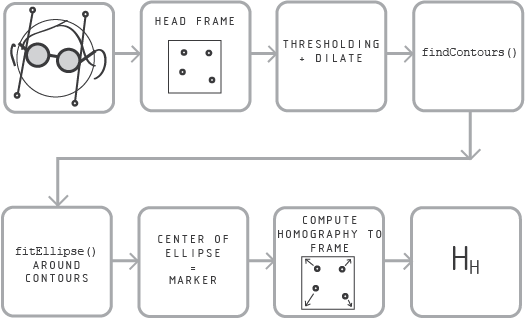
\includegraphics[width=0.9\textwidth]{03.png}
  \end{center}
\end{frame}
\subsubsection{Eye Tracking}
\begin{frame}
	\frametitle{Software}
  \framesubtitle{Eye Tracking}
  \vspace*{-0.5cm}
  \begin{center}
    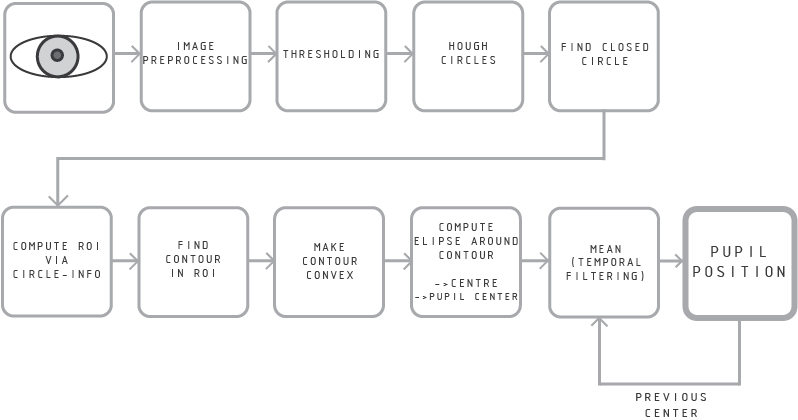
\includegraphics[width=1.05\textwidth]{02.png}
  \end{center}
\end{frame}



\subsection{Basic idea}
\subsubsection{The math}
\begin{frame}
	\frametitle{Basic idea}
  \framesubtitle{The ``math''}
  \begin{block}{Basic idea}
    \begin{equation*}
      x_\mathrm{screen} = H x_\mathrm{eye}
    \end{equation*}
  \end{block}\pause
  \begin{block}{Calibration}
    \begin{equation*}
      x_\mathrm{screen} = H_\mathrm{calib} (H_\mathrm{calib-head} x_\mathrm{eye})
    \end{equation*}
  \end{block}\pause
  \begin{block}{Calibrated mapping}
    \begin{equation*}
      H_\mathrm{calib} = H_\mathrm{eye} H_\mathrm{calib-head} ^{-1}
    \end{equation*}
  \end{block}
\end{frame}

\begin{frame}
	\frametitle{Basic idea}
  \framesubtitle{The ``math''}
  \begin{block}{Mapping without head movement}
    \begin{equation*}
      x_\mathrm{screen} = H_\mathrm{eye} H_\mathrm{calib-head} ^{-1} H_\mathrm{calib-head} x_\mathrm{eye}
    \end{equation*}
    \begin{equation*}
      x_\mathrm{screen} = H_\mathrm{eye}  x_\mathrm{eye}
    \end{equation*}
  \end{block}\pause
  \begin{block}{Mapping with head movement}
    \begin{equation*}
      x_\mathrm{screen} = H_\mathrm{eye} H_\mathrm{calib-head} ^{-1} H_\mathrm{head} x_\mathrm{eye}
    \end{equation*}
    \begin{equation*}
      H_\mathrm{rel-head} = H_\mathrm{calib-head}^{-1} H_\mathrm{head}
    \end{equation*}
  \end{block}
\end{frame}

\begin{frame}
	\frametitle{Basic idea}
  \framesubtitle{The problems with the head tracking}
  \begin{itemize}
    \item problem is ill-conditioned
    \item small uncertainties have a big effect on the mapping
    \item one has to know the position of the eye frame within the frame spanned by the markers
    \item therefore all the geometries have to be known exactly
  \end{itemize}
\end{frame}

\section{Results}
\subsection{Video}
\begin{frame}
	\frametitle{Results}
  \framesubtitle{Video}
\end{frame}

\section{Discussion}
\subsection{Problems}
\begin{frame}
	\frametitle{Discussion}
  \framesubtitle{Problems}
  \begin{itemize}
    \item bad hardware
      \begin{itemize}
        \item removed IR cutoff filter $\rightarrow$ flickering
        \item bad resolution of eye camera
        \item IR cutoff filter head camera $\rightarrow$ high integration time, harder to track IR LEDs
      \end{itemize}
    \item little inaccuracies have big effect
      \begin{itemize}
        \item where is the eye frame within the markers?
        \item what is the relation of the eye frame to the markers?
      \end{itemize}
  \end{itemize}
\end{frame}
\subsection{Conclusion}
\begin{frame}
	\frametitle{Discussion}
  \framesubtitle{Conclusion}
  \begin{itemize}
    \item works in principle
    \item perfect eye tracking is crutial
    \item knowledge of the geometries is crutial as well
    \item once the geometries are known, one could imlement another calibration routine to find the relationship of the eye frame to the frame spanned by the markers
  \end{itemize}
\end{frame}


\subsection*{Thank You}
\begin{frame}
  \begin{center}
    \huge{Thank You!}
  \end{center}
\end{frame}

\end{document}
%%%%%%%%%%%%%%%%%%%%%%%%%%%%%%%%%%%%%%%%%%%%%%%%%%%%%%%%%%%%%%%%%%%%%%%%%%%%

%% EOF
